%نام و نام خانوادگی:
%شماره دانشجویی: 
\مسئله{}
جایگاه فاز طراحی در متدولوژی اسکرام \footnote{Scrum} کجاست؟ توضیح دهید.

\پاسخ{
	
پاسخ کوتاه به این سوال این است که متدولوژی اسکرام به طور مشخص فاز طراحی ندارد! در ادامه به تفصیل به توضیح این موضوع و راه‌حل‌های آن می‌پردازیم.

\begin{figure}[!ht]
	\centering
	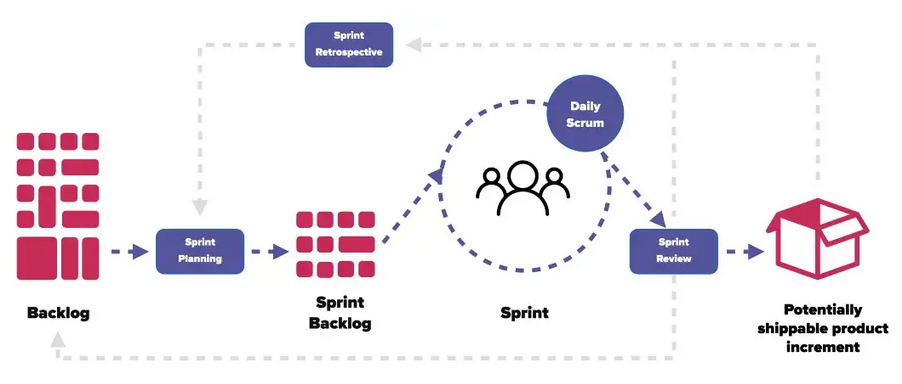
\includegraphics[scale=0.4]{figs/scrum.png}
	\caption{نمایی از متدولوژی اسکرام}	
	\label{farzamfig3}
\end{figure}

متدولوژی اسکرام راهنمایی‌هایی برای برنامه‌ریزی، تخمین، تعریف نیازمندی‌ها، پیاده‌سازی و تست را در خود دارد، اما فاز مشخصی برای طراحی یا آنالیز یا راهنمایی‌ای برای طراحی در آن وجود ندارد. 
یک راه برای گنجاندن طراحی استفاده از متدولوژی dual-track در کنار اسکرام است. در متدولوژی چابک dual-track ما دو جریان موازی داریم که اولی به پژوهش، طراحی، تست و ولیدیت کردن ایده‌ها می‌پردازد و جریان دوم ایده‌های بدست آمده از جریان اول را پیاده‌سازی و به محصول اضافه می‌کند. استفاده از این متدولوژی در کنار اسکرام به این معناست که جریان اول در هر اسپرینت بک‌لاگ اسپرینت بعدی جریان دوم را تهیه می‌کند.

\begin{figure}[!ht]
	\centering
	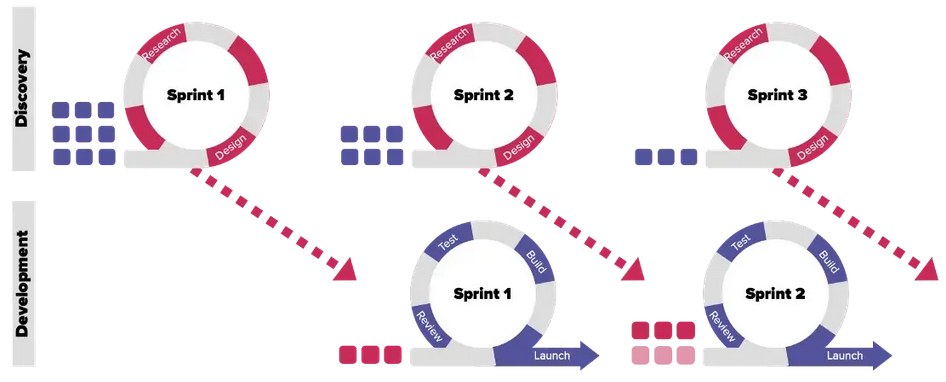
\includegraphics[scale=0.4]{figs/dual-scrum.png}
	\caption{نمایی از استفاده‌ی متدولوژی‌ dual-track در کنار اسکرام}	
	\label{farzamfig3}
\end{figure}



\subsection*{مراجع}

\begin{latin}
	\begingroup
	\renewcommand{\section}[2]{}%
	
\begin{thebibliography}{9}
%   Check this for adding items: https://www.student.unsw.edu.au/how-do-i-cite-electronic-sources
	
\bibitem{item1}
\textit{\url{https://processgroup.com/using-scrum-wisely-where-does-design-fit/}}

\bibitem{item2}
\textit{\url{https://medium.com/softserve-do/design-in-scrum-framework-d9abab28b05b}}

\end{thebibliography}
\endgroup
\end{latin}

}
\newpage
